\documentclass[11pt,ignorenonframetext,]{beamer}
\setbeamertemplate{caption}[numbered]
\setbeamertemplate{caption label separator}{: }
\setbeamercolor{caption name}{fg=normal text.fg}
\beamertemplatenavigationsymbolsempty
\usepackage{lmodern}
\usepackage{amssymb,amsmath}
\usepackage{ifxetex,ifluatex}
\usepackage{fixltx2e} % provides \textsubscript
\ifnum 0\ifxetex 1\fi\ifluatex 1\fi=0 % if pdftex
  \usepackage[T1]{fontenc}
  \usepackage[utf8]{inputenc}
\else % if luatex or xelatex
  \ifxetex
    \usepackage{mathspec}
  \else
    \usepackage{fontspec}
  \fi
  \defaultfontfeatures{Ligatures=TeX,Scale=MatchLowercase}
\fi
\usetheme[]{metropolis}
% use upquote if available, for straight quotes in verbatim environments
\IfFileExists{upquote.sty}{\usepackage{upquote}}{}
% use microtype if available
\IfFileExists{microtype.sty}{%
\usepackage{microtype}
\UseMicrotypeSet[protrusion]{basicmath} % disable protrusion for tt fonts
}{}
\newif\ifbibliography
\hypersetup{
            pdftitle={Lecture 6},
            pdfauthor={Colin Rundel},
            pdfborder={0 0 0},
            breaklinks=true}
\urlstyle{same}  % don't use monospace font for urls
\usepackage{color}
\usepackage{fancyvrb}
\newcommand{\VerbBar}{|}
\newcommand{\VERB}{\Verb[commandchars=\\\{\}]}
\DefineVerbatimEnvironment{Highlighting}{Verbatim}{commandchars=\\\{\}}
% Add ',fontsize=\small' for more characters per line
\newenvironment{Shaded}{}{}
\newcommand{\KeywordTok}[1]{\textcolor[rgb]{0.00,0.44,0.13}{\textbf{#1}}}
\newcommand{\DataTypeTok}[1]{\textcolor[rgb]{0.56,0.13,0.00}{#1}}
\newcommand{\DecValTok}[1]{\textcolor[rgb]{0.25,0.63,0.44}{#1}}
\newcommand{\BaseNTok}[1]{\textcolor[rgb]{0.25,0.63,0.44}{#1}}
\newcommand{\FloatTok}[1]{\textcolor[rgb]{0.25,0.63,0.44}{#1}}
\newcommand{\ConstantTok}[1]{\textcolor[rgb]{0.53,0.00,0.00}{#1}}
\newcommand{\CharTok}[1]{\textcolor[rgb]{0.25,0.44,0.63}{#1}}
\newcommand{\SpecialCharTok}[1]{\textcolor[rgb]{0.25,0.44,0.63}{#1}}
\newcommand{\StringTok}[1]{\textcolor[rgb]{0.25,0.44,0.63}{#1}}
\newcommand{\VerbatimStringTok}[1]{\textcolor[rgb]{0.25,0.44,0.63}{#1}}
\newcommand{\SpecialStringTok}[1]{\textcolor[rgb]{0.73,0.40,0.53}{#1}}
\newcommand{\ImportTok}[1]{#1}
\newcommand{\CommentTok}[1]{\textcolor[rgb]{0.38,0.63,0.69}{\textit{#1}}}
\newcommand{\DocumentationTok}[1]{\textcolor[rgb]{0.73,0.13,0.13}{\textit{#1}}}
\newcommand{\AnnotationTok}[1]{\textcolor[rgb]{0.38,0.63,0.69}{\textbf{\textit{#1}}}}
\newcommand{\CommentVarTok}[1]{\textcolor[rgb]{0.38,0.63,0.69}{\textbf{\textit{#1}}}}
\newcommand{\OtherTok}[1]{\textcolor[rgb]{0.00,0.44,0.13}{#1}}
\newcommand{\FunctionTok}[1]{\textcolor[rgb]{0.02,0.16,0.49}{#1}}
\newcommand{\VariableTok}[1]{\textcolor[rgb]{0.10,0.09,0.49}{#1}}
\newcommand{\ControlFlowTok}[1]{\textcolor[rgb]{0.00,0.44,0.13}{\textbf{#1}}}
\newcommand{\OperatorTok}[1]{\textcolor[rgb]{0.40,0.40,0.40}{#1}}
\newcommand{\BuiltInTok}[1]{#1}
\newcommand{\ExtensionTok}[1]{#1}
\newcommand{\PreprocessorTok}[1]{\textcolor[rgb]{0.74,0.48,0.00}{#1}}
\newcommand{\AttributeTok}[1]{\textcolor[rgb]{0.49,0.56,0.16}{#1}}
\newcommand{\RegionMarkerTok}[1]{#1}
\newcommand{\InformationTok}[1]{\textcolor[rgb]{0.38,0.63,0.69}{\textbf{\textit{#1}}}}
\newcommand{\WarningTok}[1]{\textcolor[rgb]{0.38,0.63,0.69}{\textbf{\textit{#1}}}}
\newcommand{\AlertTok}[1]{\textcolor[rgb]{1.00,0.00,0.00}{\textbf{#1}}}
\newcommand{\ErrorTok}[1]{\textcolor[rgb]{1.00,0.00,0.00}{\textbf{#1}}}
\newcommand{\NormalTok}[1]{#1}
\usepackage{graphicx,grffile}
\makeatletter
\def\maxwidth{\ifdim\Gin@nat@width>\linewidth\linewidth\else\Gin@nat@width\fi}
\def\maxheight{\ifdim\Gin@nat@height>\textheight0.8\textheight\else\Gin@nat@height\fi}
\makeatother
% Scale images if necessary, so that they will not overflow the page
% margins by default, and it is still possible to overwrite the defaults
% using explicit options in \includegraphics[width, height, ...]{}
\setkeys{Gin}{width=\maxwidth,height=\maxheight,keepaspectratio}

% Prevent slide breaks in the middle of a paragraph:
\widowpenalties 1 10000
\raggedbottom

\AtBeginPart{
  \let\insertpartnumber\relax
  \let\partname\relax
  \frame{\partpage}
}
\AtBeginSection{
  \ifbibliography
  \else
    \let\insertsectionnumber\relax
    \let\sectionname\relax
    \frame{\sectionpage}
  \fi
}
\AtBeginSubsection{
  \let\insertsubsectionnumber\relax
  \let\subsectionname\relax
  \frame{\subsectionpage}
}

\setlength{\parindent}{0pt}
\setlength{\parskip}{6pt plus 2pt minus 1pt}
\setlength{\emergencystretch}{3em}  % prevent overfull lines
\providecommand{\tightlist}{%
  \setlength{\itemsep}{0pt}\setlength{\parskip}{0pt}}
\setcounter{secnumdepth}{0}

\usepackage{geometry}
\usepackage{graphicx}
\usepackage{amssymb}
\usepackage{color}          	% gives color options
\usepackage{url}		% produces hyperlinks
\usepackage[english]{babel}
\usepackage{colortbl}	% allows for color usage in tables
\usepackage{multirow}	% allows for rows that span multiple rows in tables
\usepackage{xcolor}		% this package has a variety of color options
\usepackage{calc}
\usepackage{multicol}
\usepackage{wrapfig}
\usepackage{textcomp}
\usepackage{bm}
\usepackage{bbm}
\usepackage{setspace}
\singlespacing

%%%%%%%%%%%%%%%%
% Small code output
%%%%%%%%%%%%%%%%

%% change fontsize of R code
\let\oldShaded\Shaded
\let\endoldShaded\endShaded
\renewenvironment{Shaded}{\footnotesize\begin{spacing}{0.9}\oldShaded}{\endoldShaded\end{spacing}}

%% change fontsize of output
\let\oldverbatim\verbatim
\let\endoldverbatim\endverbatim
\renewenvironment{verbatim}{\footnotesize\begin{spacing}{0.9}\oldverbatim}{\endoldverbatim\end{spacing}}


\newcommand{\verbatimfont}[1]{\renewcommand{\verbatim@font}{\ttfamily#1}}

%%%%%%%%%%%%%%%%
% Custom Colors
%%%%%%%%%%%%%%%%

\xdefinecolor{oiBlue}{rgb}{0.15, 0.35, 0.55}
\xdefinecolor{gray}{rgb}{0.5, 0.5, 0.5}
\xdefinecolor{darkGray}{rgb}{0.3, 0.3, 0.3}
\xdefinecolor{darkerGray}{rgb}{0.2, 0.2, 0.2}
\xdefinecolor{rubineRed}{rgb}{0.89,0,0.30}
\xdefinecolor{linkCol}{rgb}{0.11,0.49,0.95}	
\xdefinecolor{irishGreen}{rgb}{0,0.60,0}	
\xdefinecolor{darkturquoise}{rgb}{0.44, 0.58, 0.86}
\definecolor{lightGreen}{rgb}{0.533,0.765,0.42}
%\xdefinecolor{hlblue}{rgb}{0.051,0.65,1}
\xdefinecolor{hlblue}{rgb}{ 0.055, 0.639, 0.831}
\definecolor{light}{rgb}{.337,.608,.741}
\definecolor{dark}{rgb}{.337,.608,.741}

\definecolor{cpink}{rgb}{0.93, 0.23, 0.51}

%%%%%%%%%%%%%%%%
% Custom Commands
%%%%%%%%%%%%%%%%

% text colors
\newcommand{\red}[1]{\textit{\textcolor{rubineRed}{#1}}}
\newcommand{\orange}[1]{\textit{\textcolor{orange}{#1}}}
\newcommand{\pink}[1]{\textit{\textcolor{rubineRed!90!white!50}{#1}}}
\newcommand{\green}[1]{\textit{\textcolor{irishGreen}{#1}}}
\newcommand{\blue}[1]{\textit{\textcolor{darkturquoise}{#1}}}
\newcommand{\light}[1]{\textcolor{light}{\textbf{#1}}}
\newcommand{\dark}[1]{\textcolor{dark}{#1}}
\newcommand{\gray}[1]{\textcolor{gray}{#1}}


% links: webURL, webLin, appLink
\newcommand{\webURL}[1]{\urlstyle{same}{\textit{\textcolor{linkCol}{\url{#1}}} }}
\newcommand{\webLink}[2]{\href{#1}{\textcolor{linkCol}{{#2}}}}
\newcommand{\appLink}[2]{\href{#1}{\textcolor{lightGreen!80!black!90}{{#2}}}}

% mail
\newcommand{\mail}[1]{\href{mailto:#1}{\textit{\textcolor{linkCol}{#1}}}}

% highlighting: hl, hlGr, mathhl
\newcommand{\hl}[1]{\textit{\textcolor{hlblue}{#1}}}
\newcommand{\hlGr}[1]{\textit{\textcolor{lightGreen}{#1}}}
\newcommand{\hlRd}[1]{\textit{\textcolor{rubineRed}{#1}}}
\newcommand{\mathhl}[1]{\textcolor{hlblue}{\ensuremath{#1}}}

% example
\newcommand{\ex}[1]{\textcolor{blue}{{{\small (#1)}}}}


\DeclareMathOperator*{\argmin}{arg\,min}
\DeclareMathOperator*{\argmax}{arg\,max}

\title{Lecture 6}
\subtitle{Discrete Time Series}
\author{Colin Rundel}
\date{02/06/2017}

\begin{document}
\frame{\titlepage}

\section{Discrete Time Series}\label{discrete-time-series}

\begin{frame}[t]{Stationary Processes}

A stocastic process (i.e.~a time series) is considered to be
\emph{strictly stationary} if the properties of the process are not
changed by a shift in origin.

\pause

In the time series context this means that the joint distribution of
\(\{y_{t_1}, \ldots, y_{t_n}\}\) must be identical to the distribution
of \(\{y_{t_1+k}, \ldots, y_{t_n+k}\}\) for any value of \(n\) and
\(k\).

\pause

\end{frame}

\begin{frame}[t]{Weak Stationary}

Strict stationary is too strong for most applications, so instead we
often opt for \emph{weak stationary} which requires the following,

\begin{enumerate}
\def\labelenumi{\arabic{enumi}.}
\item
  The process has finite variance
  \[E(y_t^2) < \infty \text{ for all $t$}\]
\item
  The mean of the process in constant
  \[E(y_t) = \mu \text{ for all $t$}\]
\item
  The second moment only depends on the lag
  \[Cov(y_t,y_s) = Cov(y_{t+k},y_{s+k}) \text{ for all $t,s,k$}\]
\end{enumerate}

\pause

When we say stationary in class we almost always mean this version of
\emph{weakly stationary}.

\end{frame}

\begin{frame}[t]{Autocorrelation}

For a stationary time series, where \(E(y_t)=\mu\) and
\(\text{Var}(y_t)=\sigma^2)\) for all \(t\), we define the
autocorrelation at lag \(k\) as

\[
\begin{aligned}
\rho_k &= Cor(y_t, \, y_{t+k}) \\
       &= \frac{Cov(y_t, y_{t+k})}{\sqrt{Var(y_t)Var(y_{t+k})}} \\
       &= \frac{E\left( (y_t-\mu)(y_{t+k}-\mu) \right)}{\sigma^2}
\end{aligned}
\]

\pause

this is also sometimes written in terms of the autocovariance function
(\(\gamma_k\)) as

\[
\begin{aligned}
\gamma_k &= \gamma(t,t+k) = Cov(y_t, y_{t+k}) \\
\rho_k &= \frac{\gamma(t,t+k)}{\sqrt{\gamma(t,t) \gamma(t+k,t+k)}} = \frac{\gamma(k)}{\gamma(0)}
\end{aligned}
\]

\end{frame}

\begin{frame}{Covariance Structure}

Based on our definition of a (weakly) stationary process, it implies a
covariance of the following structure,

\[
\left(
\begin{matrix}
\gamma(0) & \gamma(1) & \gamma(2) & \gamma(3) & \cdots & \gamma(n) \\
\gamma(1) & \gamma(0) & \gamma(1) & \gamma(2) & \cdots & \gamma(n-1) \\
\gamma(2) & \gamma(1) & \gamma(0) & \gamma(1) & \cdots & \gamma(n-2) \\
\gamma(3) & \gamma(2) & \gamma(1) & \gamma(0) & \cdots & \gamma(n-3) \\
\vdots    & \vdots    & \vdots    & \vdots    & \ddots & \vdots \\
\gamma(n) & \gamma(n-1) & \gamma(n-2) & \gamma(n-3) & \cdots & \gamma(0)
\end{matrix}
\right)
\]

\end{frame}

\begin{frame}[t]{Example - Random walk}

Let \(y_t = y_{t-1} + w_t\) with \(y_0=0\) and
\(w_t \sim \mathcal{N}(0,1)\). Is \(y_t\) stationary?

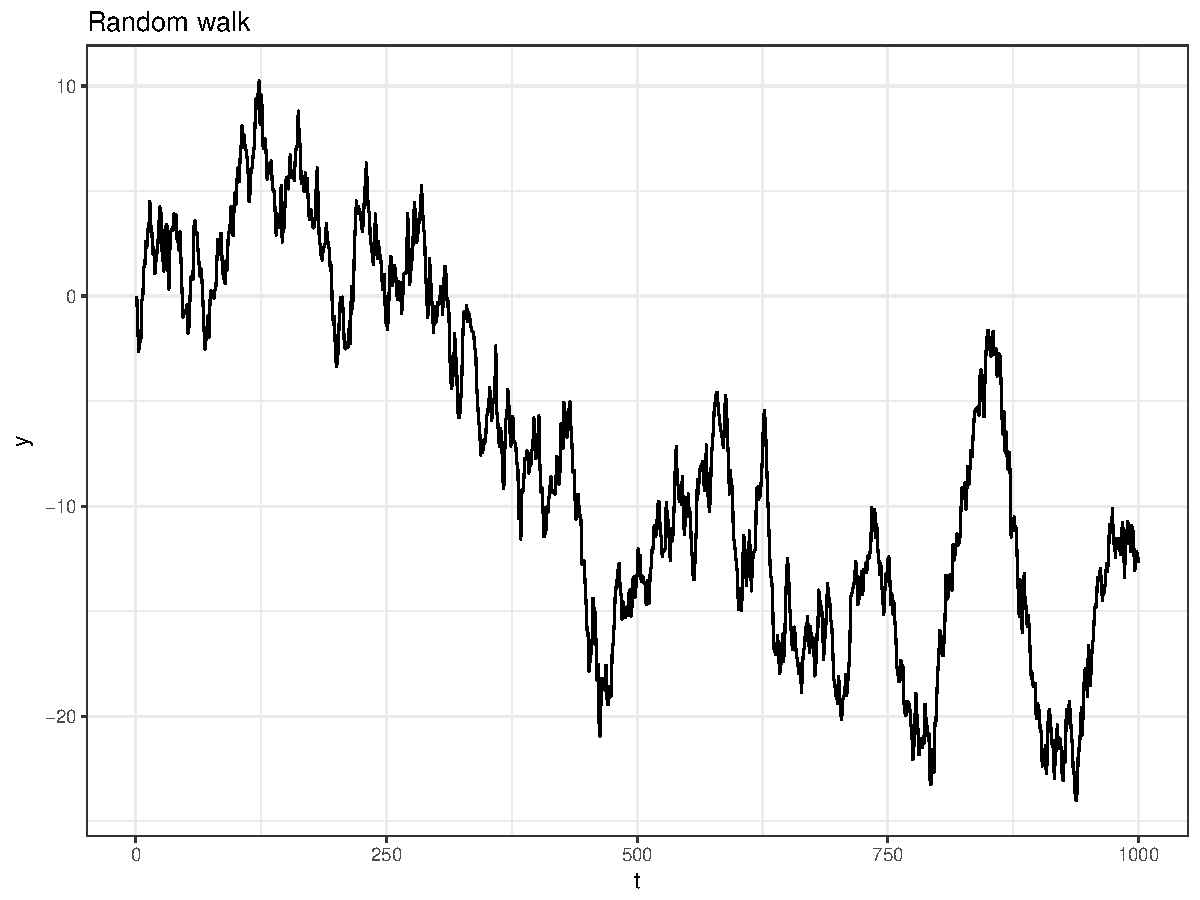
\includegraphics{Lec6_files/figure-beamer/unnamed-chunk-1-1.pdf}

\end{frame}

\begin{frame}{ACF + PACF}

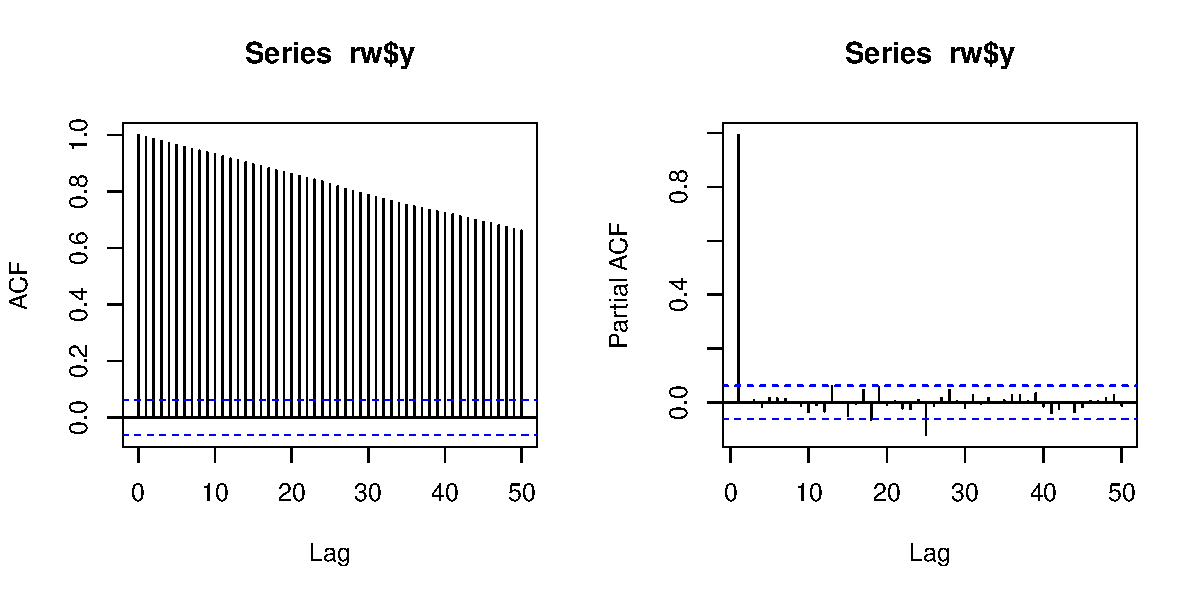
\includegraphics{Lec6_files/figure-beamer/unnamed-chunk-2-1.pdf}

\end{frame}

\begin{frame}[t]{Example - Random walk with drift}

Let \(y_t = \delta + y_{t-1} + w_t\) with \(y_0=0\) and
\(w_t \sim \mathcal{N}(0,1)\). Is \(y_t\) stationary?

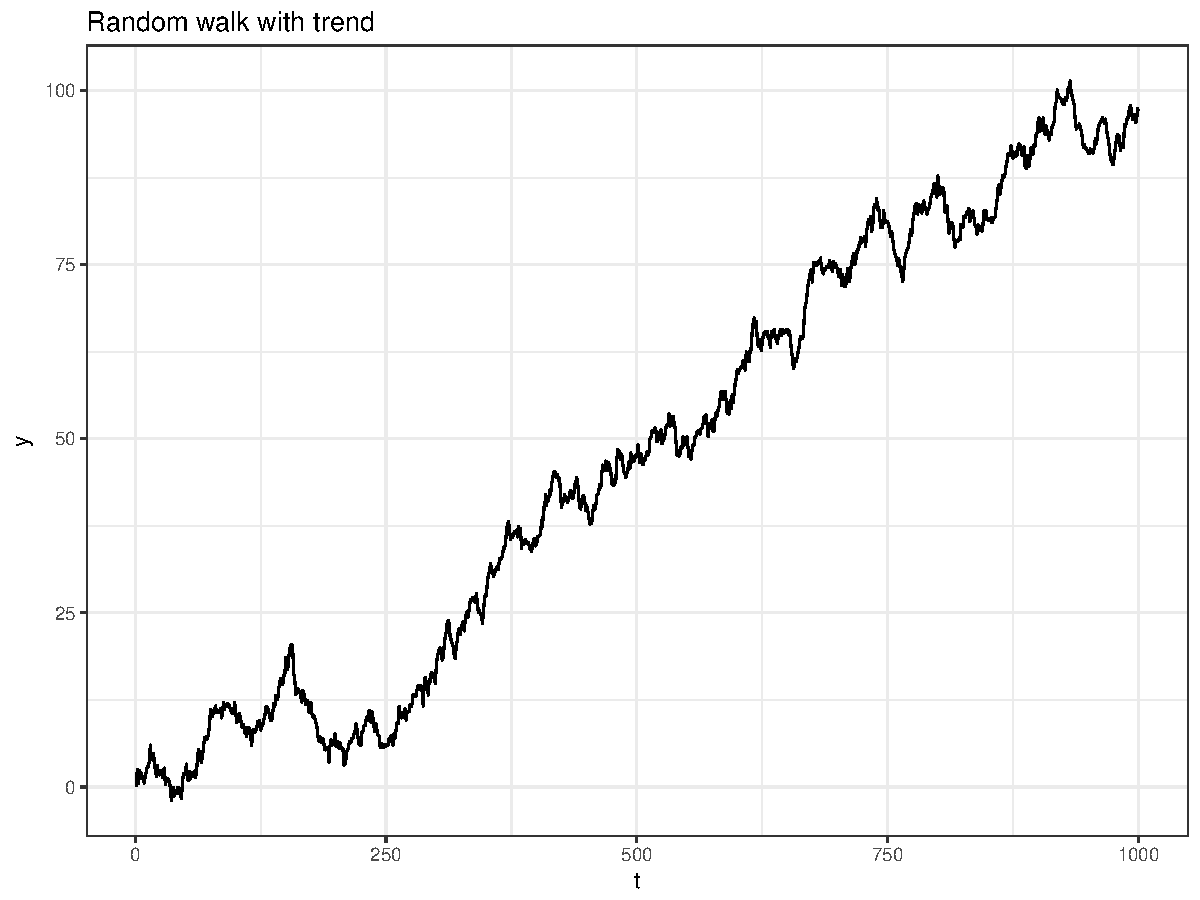
\includegraphics{Lec6_files/figure-beamer/unnamed-chunk-3-1.pdf}

\end{frame}

\begin{frame}{ACF + PACF}

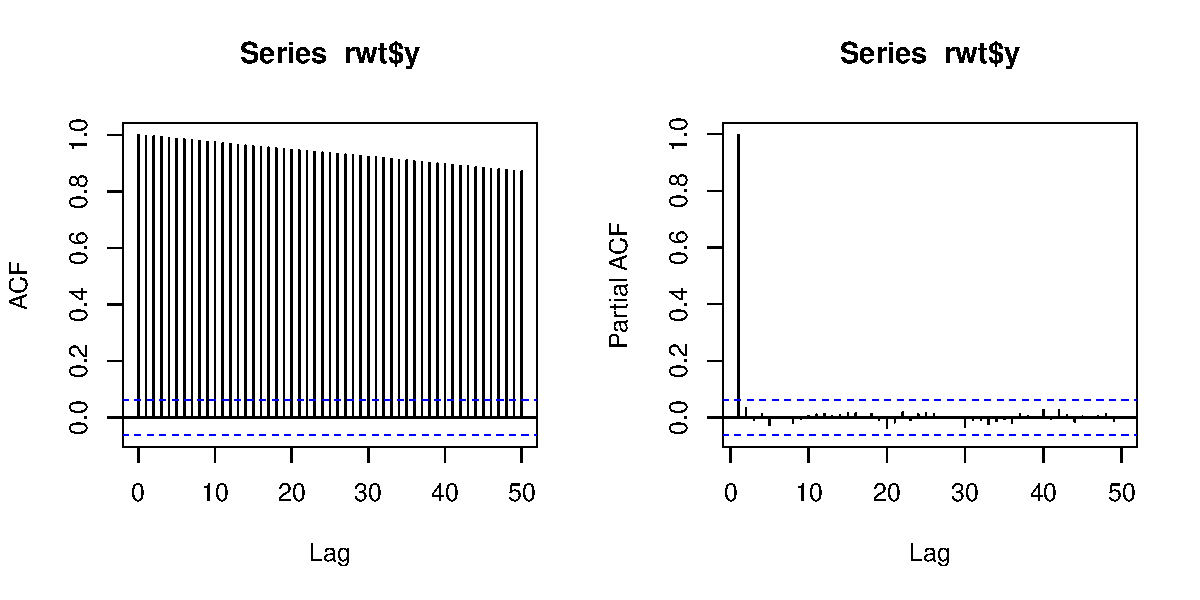
\includegraphics{Lec6_files/figure-beamer/unnamed-chunk-4-1.pdf}

\end{frame}

\begin{frame}{Example - Moving Average}

Let \(w_t \sim \mathcal{N}(0,1)\) and
\(y_t = \frac{1}{3}\left(w_{t-1}+w_t+w_{t+1}\right)\), is \(y_t\)
stationary?

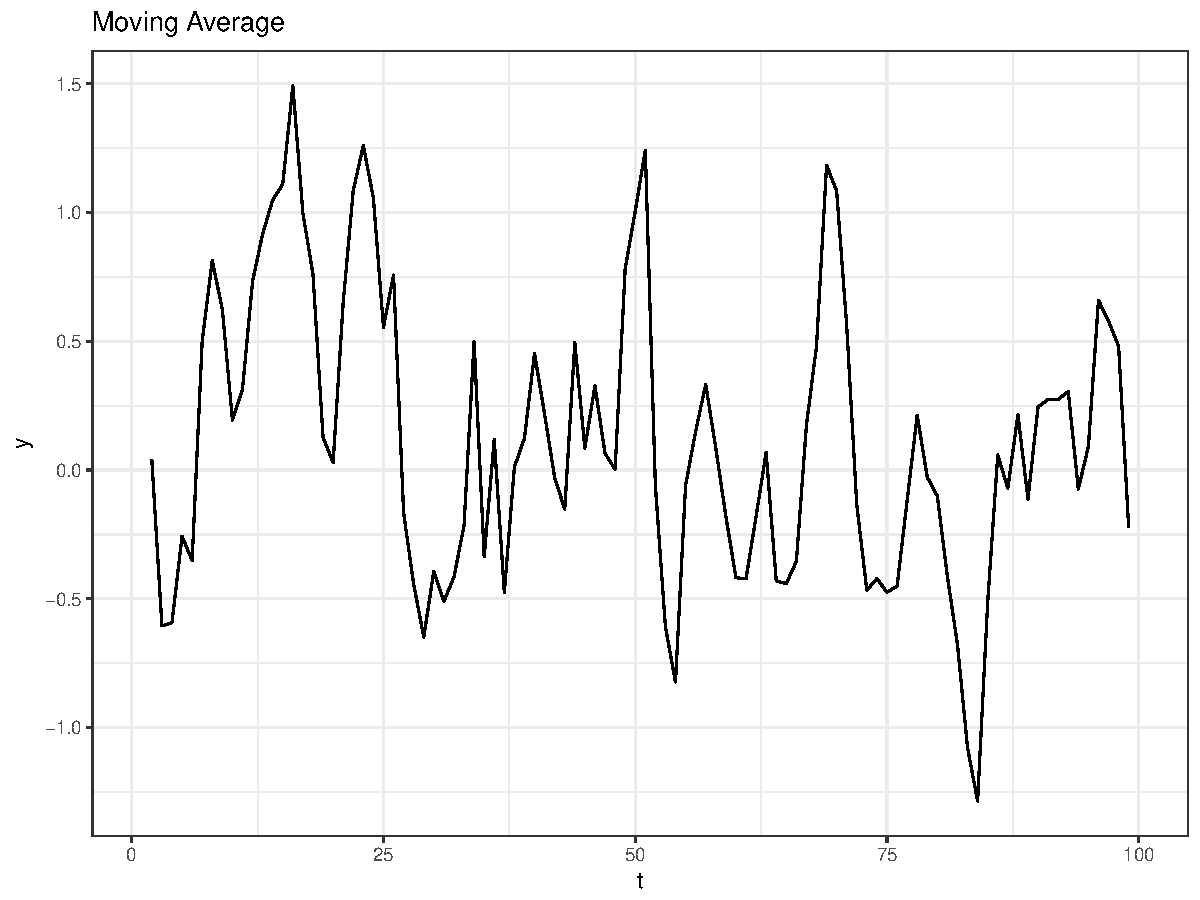
\includegraphics{Lec6_files/figure-beamer/unnamed-chunk-5-1.pdf}

\end{frame}

\begin{frame}{ACF + PACF}

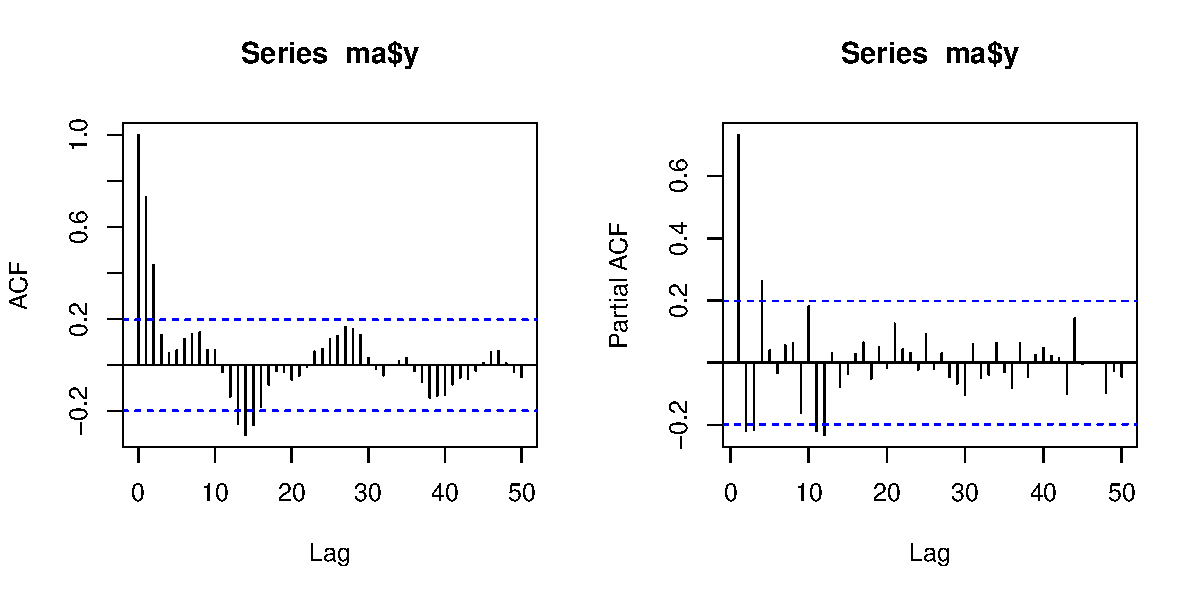
\includegraphics{Lec6_files/figure-beamer/unnamed-chunk-6-1.pdf}

\end{frame}

\begin{frame}{Autoregression}

Let \(w_t \sim \mathcal{N}(0,1)\) and
\(y_t = y_{t-1} - 0.9 y_{t-2} + w_t\) with \(y_t = 0\) for \(t < 1\), is
\(y_t\) stationary?

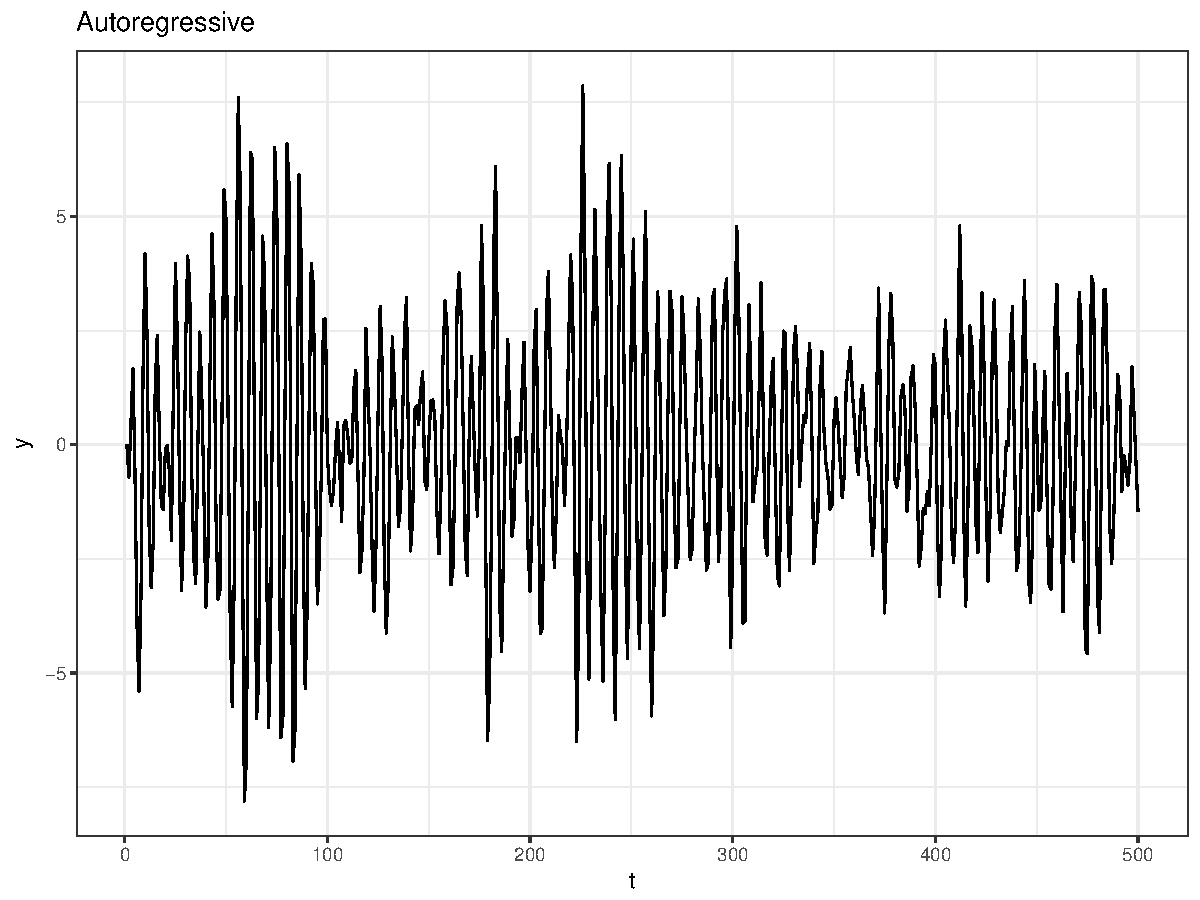
\includegraphics{Lec6_files/figure-beamer/unnamed-chunk-7-1.pdf}

\end{frame}

\begin{frame}{ACF + PACF}

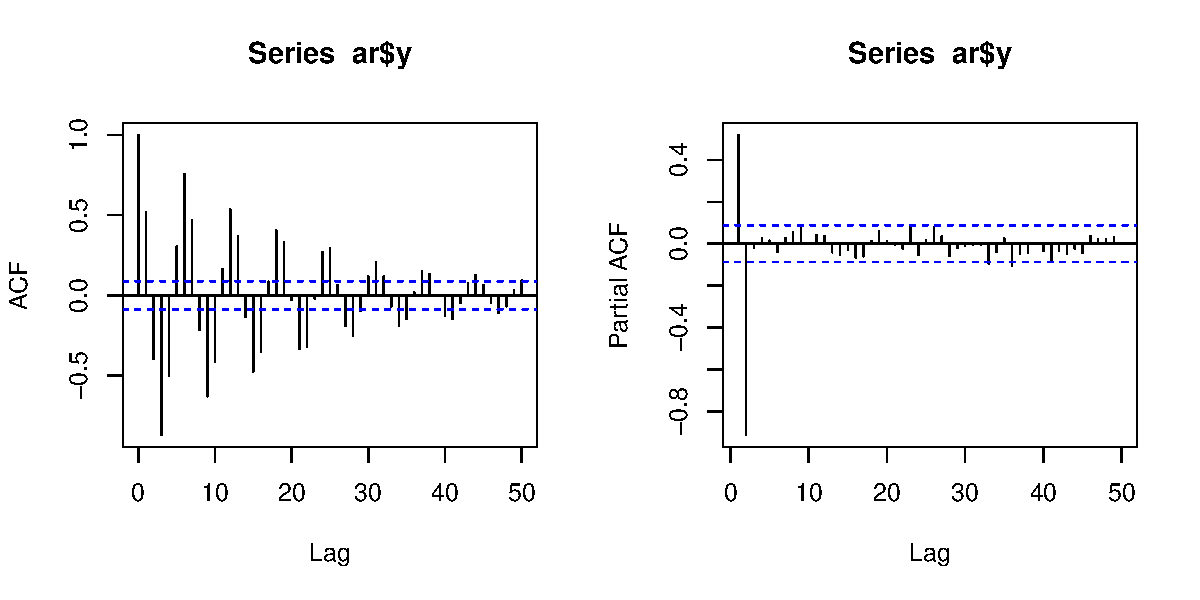
\includegraphics{Lec6_files/figure-beamer/unnamed-chunk-8-1.pdf}

\end{frame}

\begin{frame}[fragile]{Example - Australian Wine Sales}

Australian total wine sales by wine makers in bottles \textless{}= 1
litre. Jan 1980 -- Aug 1994.

\begin{Shaded}
\begin{Highlighting}[]
\KeywordTok{load}\NormalTok{(}\KeywordTok{url}\NormalTok{(}\StringTok{"http://www.stat.duke.edu/~cr173/Sta444_Sp17/data/aus_wine.Rdata"}\NormalTok{))}
\NormalTok{aus_wine}
\NormalTok{## # A tibble: 176 × 2}
\NormalTok{##        date sales}
\NormalTok{##       <dbl> <dbl>}
\NormalTok{## 1  1980.000 15136}
\NormalTok{## 2  1980.083 16733}
\NormalTok{## 3  1980.167 20016}
\NormalTok{## 4  1980.250 17708}
\NormalTok{## 5  1980.333 18019}
\NormalTok{## 6  1980.417 19227}
\NormalTok{## 7  1980.500 22893}
\NormalTok{## 8  1980.583 23739}
\NormalTok{## 9  1980.667 21133}
\NormalTok{## 10 1980.750 22591}
\NormalTok{## # ... with 166 more rows}
\end{Highlighting}
\end{Shaded}

\end{frame}

\begin{frame}{Time series}

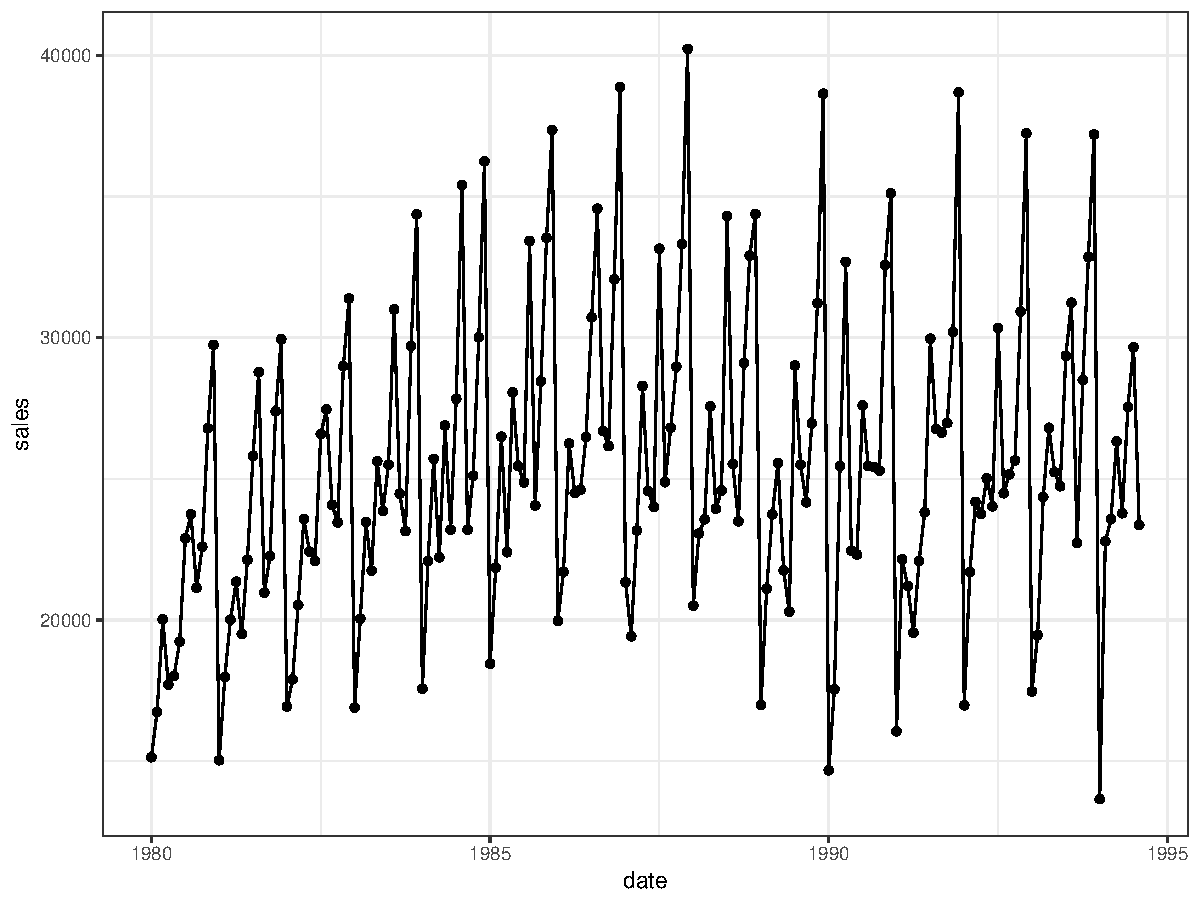
\includegraphics{Lec6_files/figure-beamer/unnamed-chunk-10-1.pdf}

\end{frame}

\begin{frame}{Basic Model Fit}

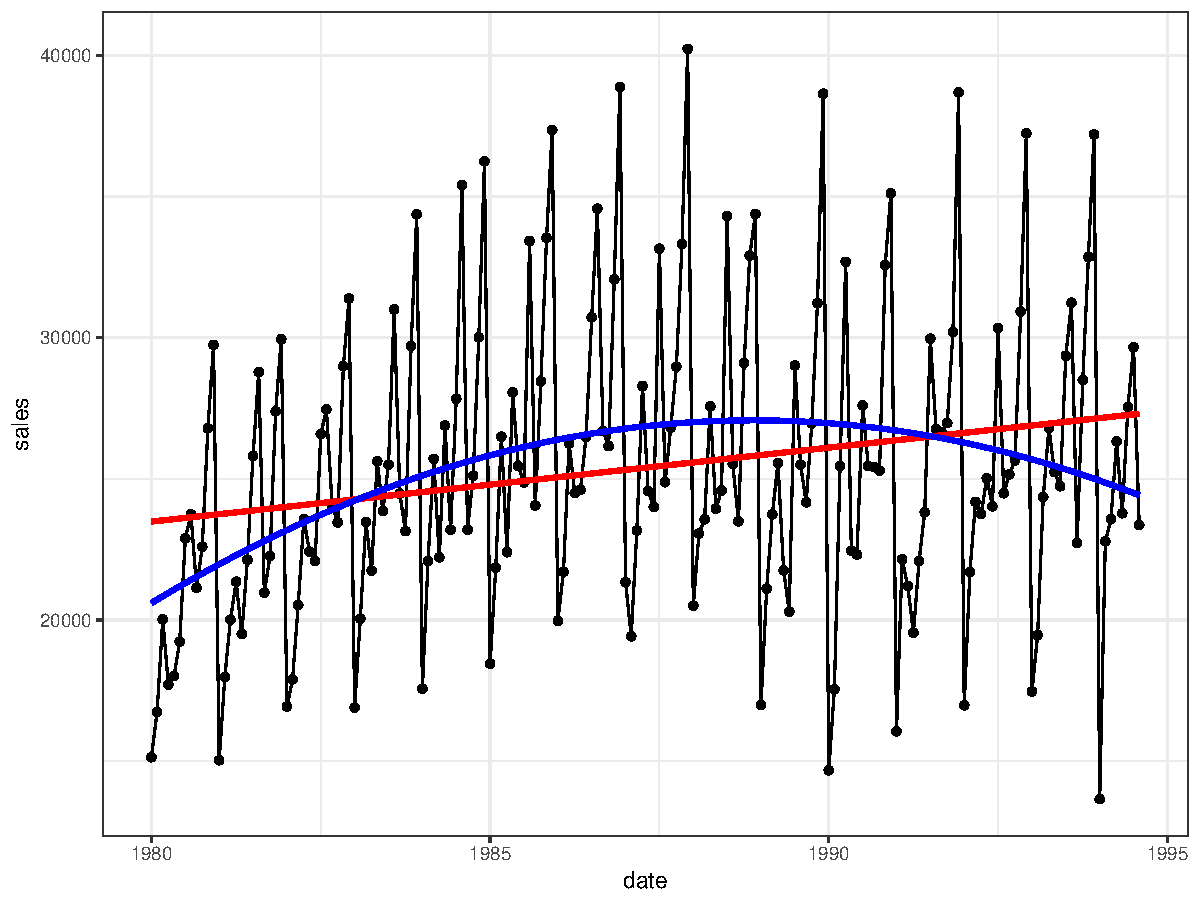
\includegraphics{Lec6_files/figure-beamer/unnamed-chunk-11-1.pdf}

\end{frame}

\begin{frame}{Residuals}

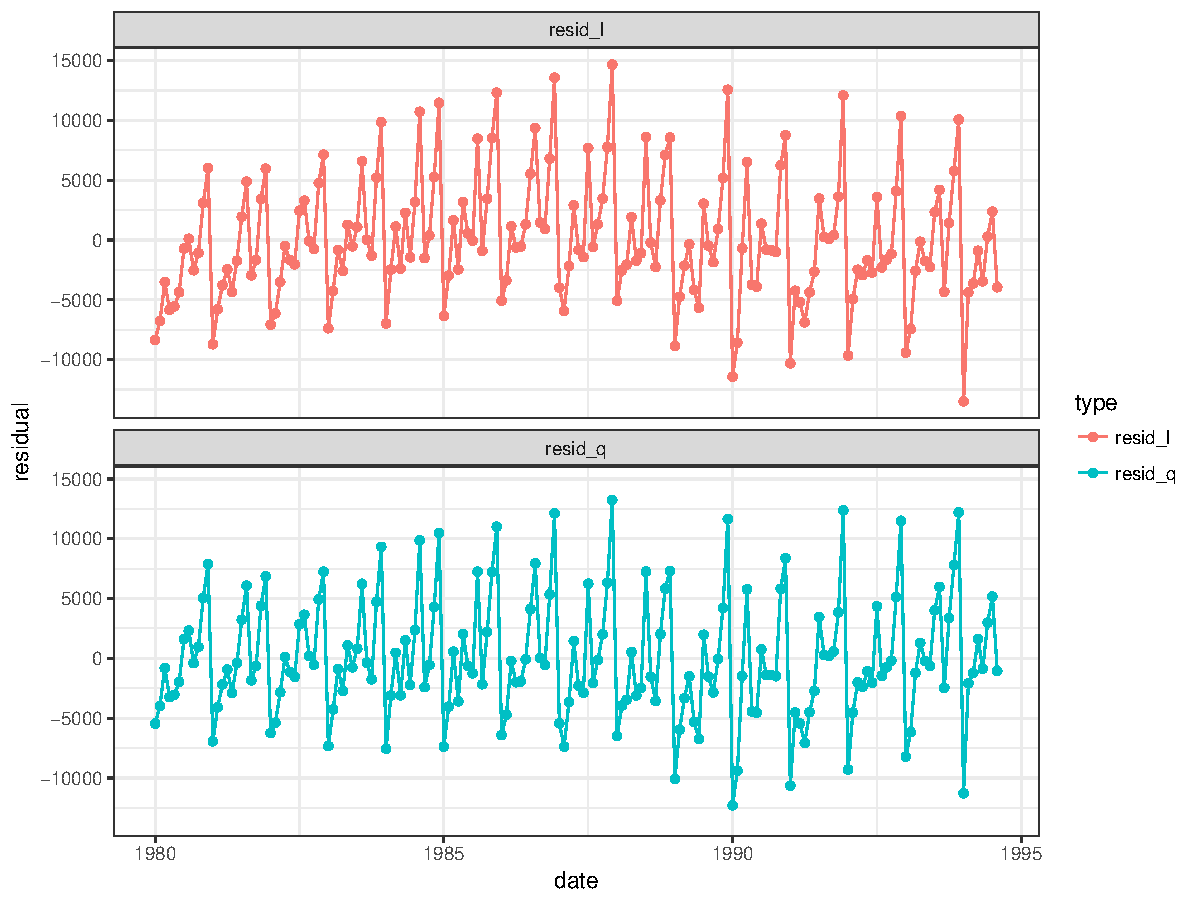
\includegraphics{Lec6_files/figure-beamer/unnamed-chunk-12-1.pdf}

\end{frame}

\begin{frame}{Autocorrelation Plot}

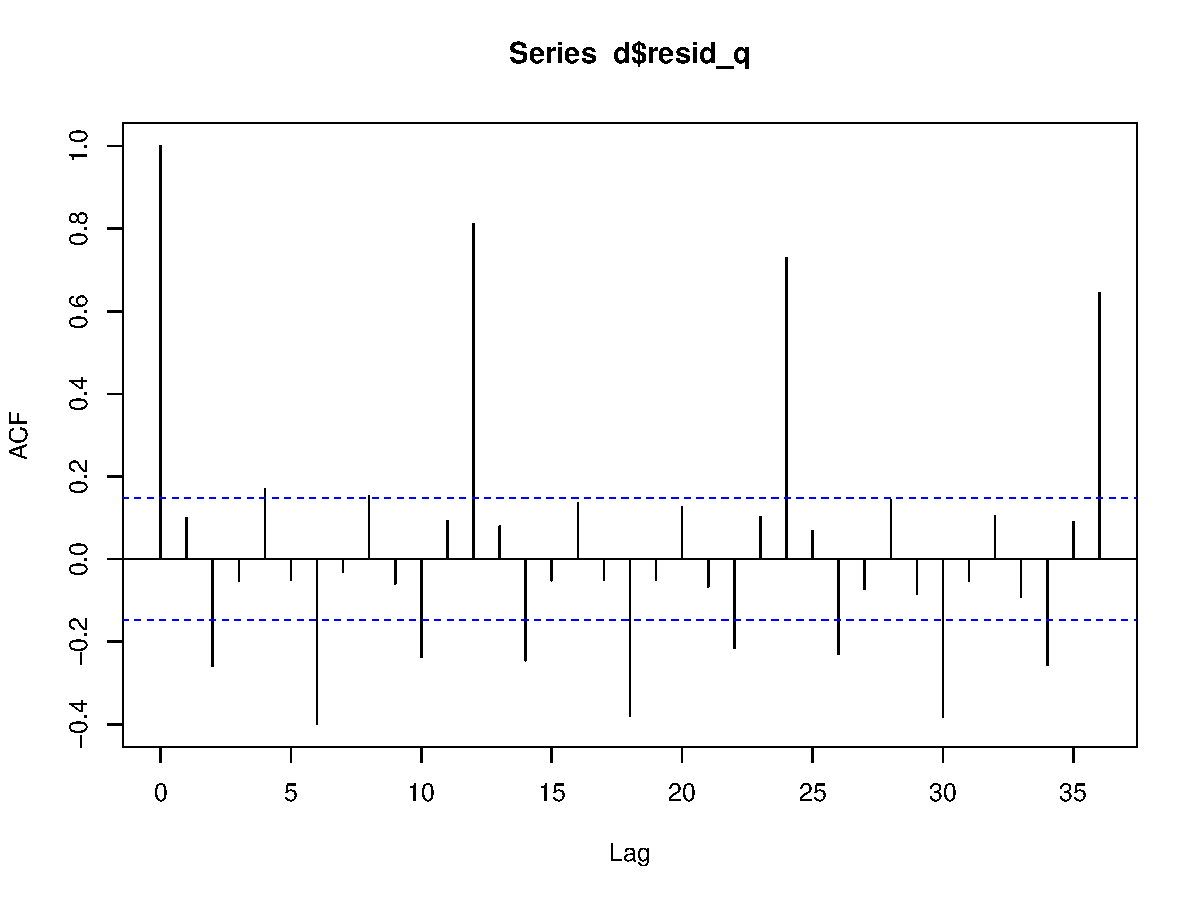
\includegraphics{Lec6_files/figure-beamer/unnamed-chunk-13-1.pdf}

\end{frame}

\begin{frame}{Partial Autocorrelation Plot}

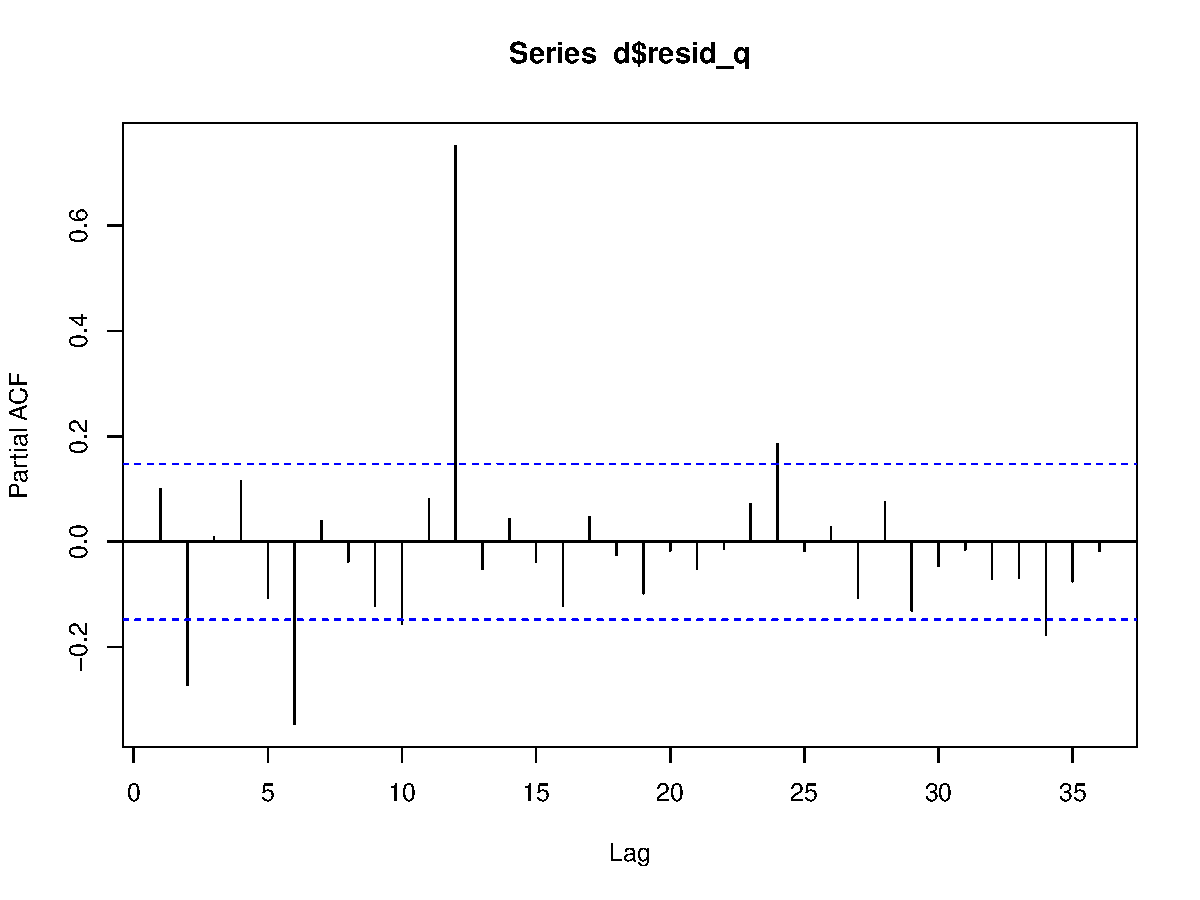
\includegraphics{Lec6_files/figure-beamer/unnamed-chunk-14-1.pdf}

\end{frame}

\begin{frame}{}

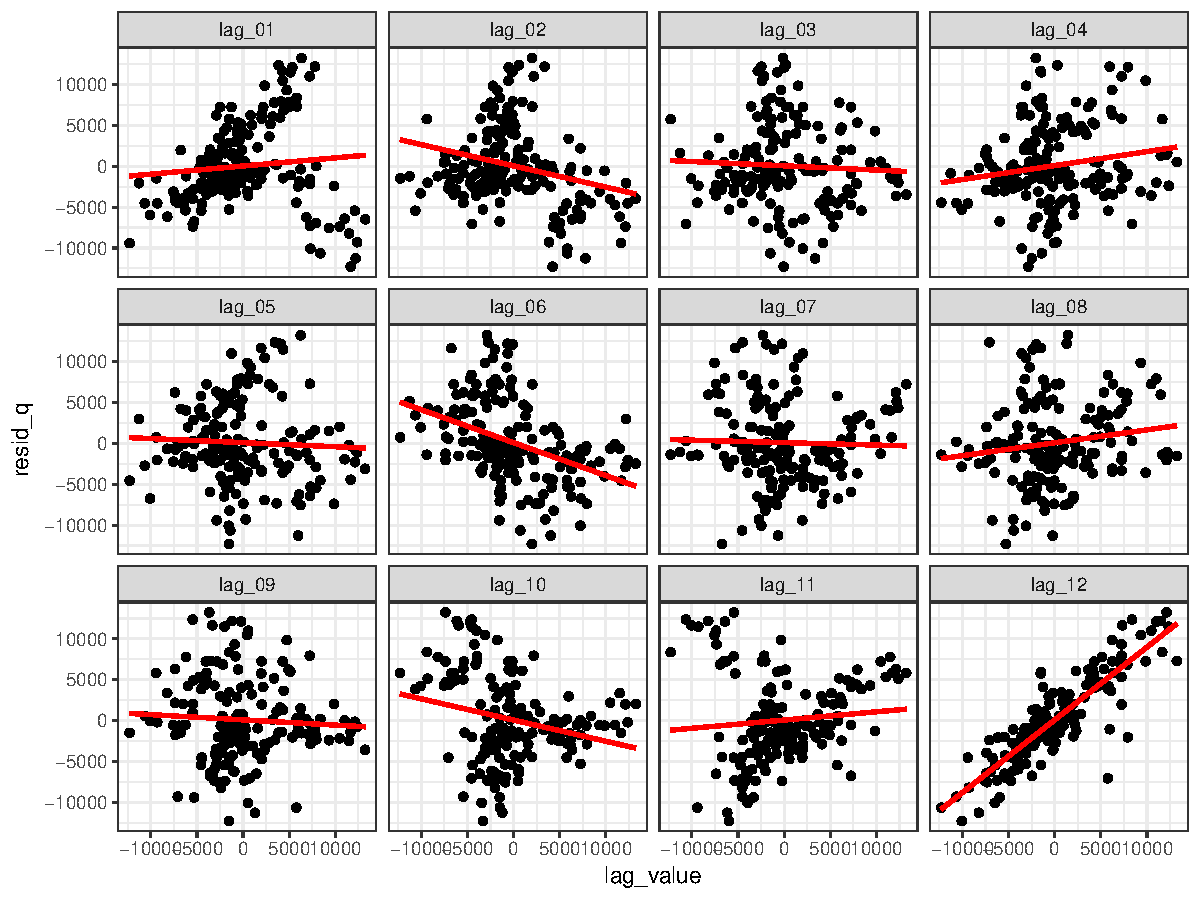
\includegraphics{Lec6_files/figure-beamer/unnamed-chunk-15-1.pdf}

\end{frame}

\begin{frame}[fragile]{Auto regressive errors}

\begin{verbatim}
## 
## Call:
## lm(formula = resid_q ~ lag_12, data = d_ar)
## 
## Residuals:
##      Min       1Q   Median       3Q      Max 
## -12286.5  -1380.5     73.4   1505.2   7188.1 
## 
## Coefficients:
##              Estimate Std. Error t value Pr(>|t|)    
## (Intercept)  83.65080  201.58416   0.415    0.679    
## lag_12        0.89024    0.04045  22.006   <2e-16 ***
## ---
## Signif. codes:  0 '***' 0.001 '**' 0.01 '*' 0.05 '.' 0.1 ' ' 1
## 
## Residual standard error: 2581 on 162 degrees of freedom
##   (12 observations deleted due to missingness)
## Multiple R-squared:  0.7493, Adjusted R-squared:  0.7478 
## F-statistic: 484.3 on 1 and 162 DF,  p-value: < 2.2e-16
\end{verbatim}

\end{frame}

\begin{frame}{Residual residuals}

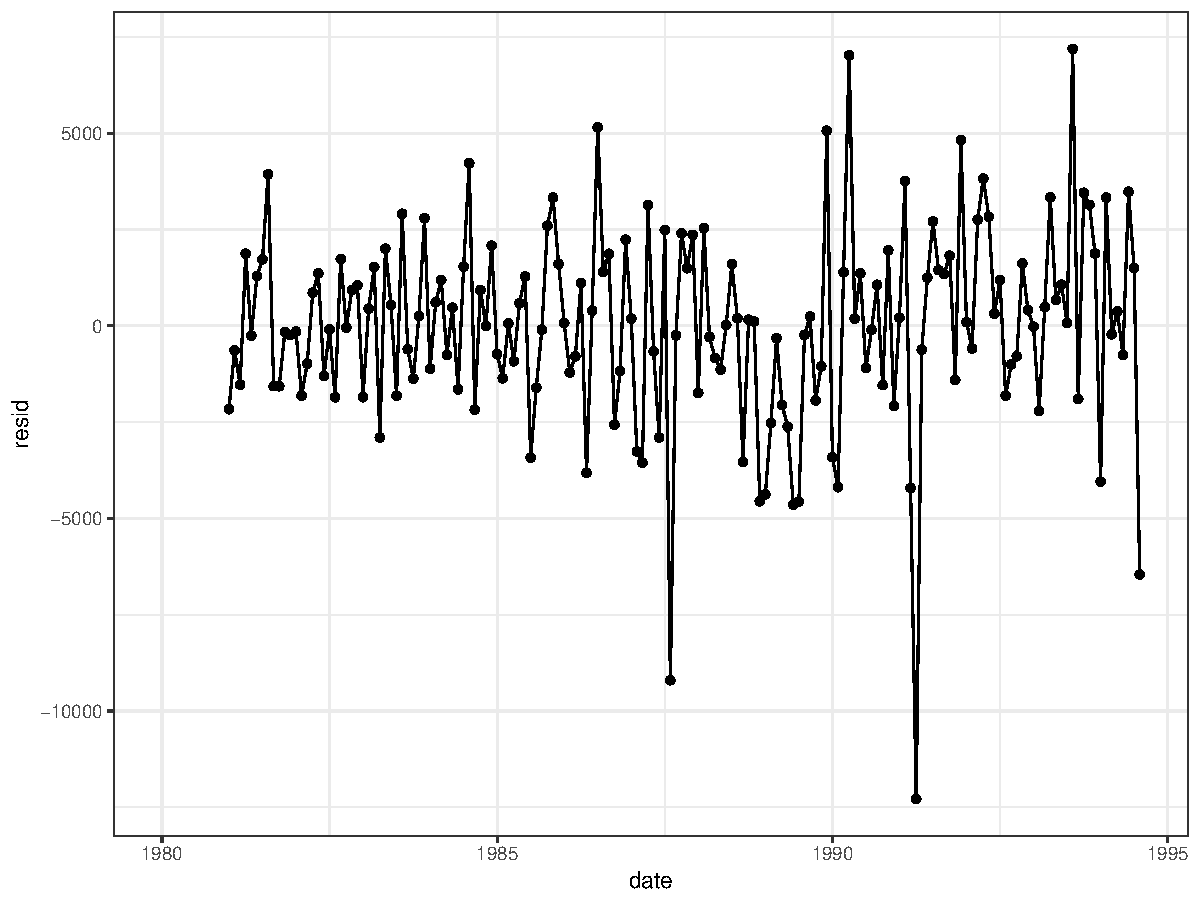
\includegraphics{Lec6_files/figure-beamer/unnamed-chunk-17-1.pdf}

\end{frame}

\begin{frame}{Residual residuals - acf}

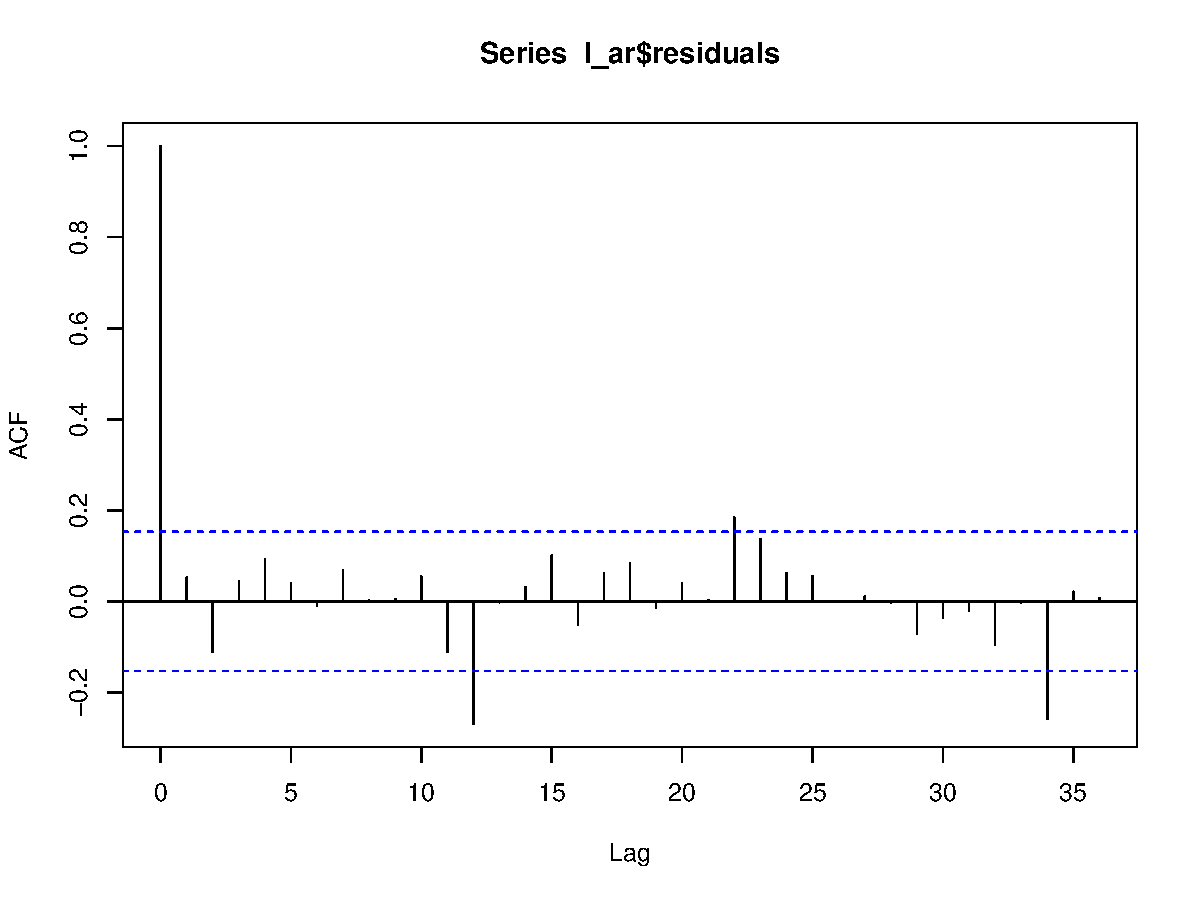
\includegraphics{Lec6_files/figure-beamer/unnamed-chunk-18-1.pdf}

\end{frame}

\begin{frame}{}

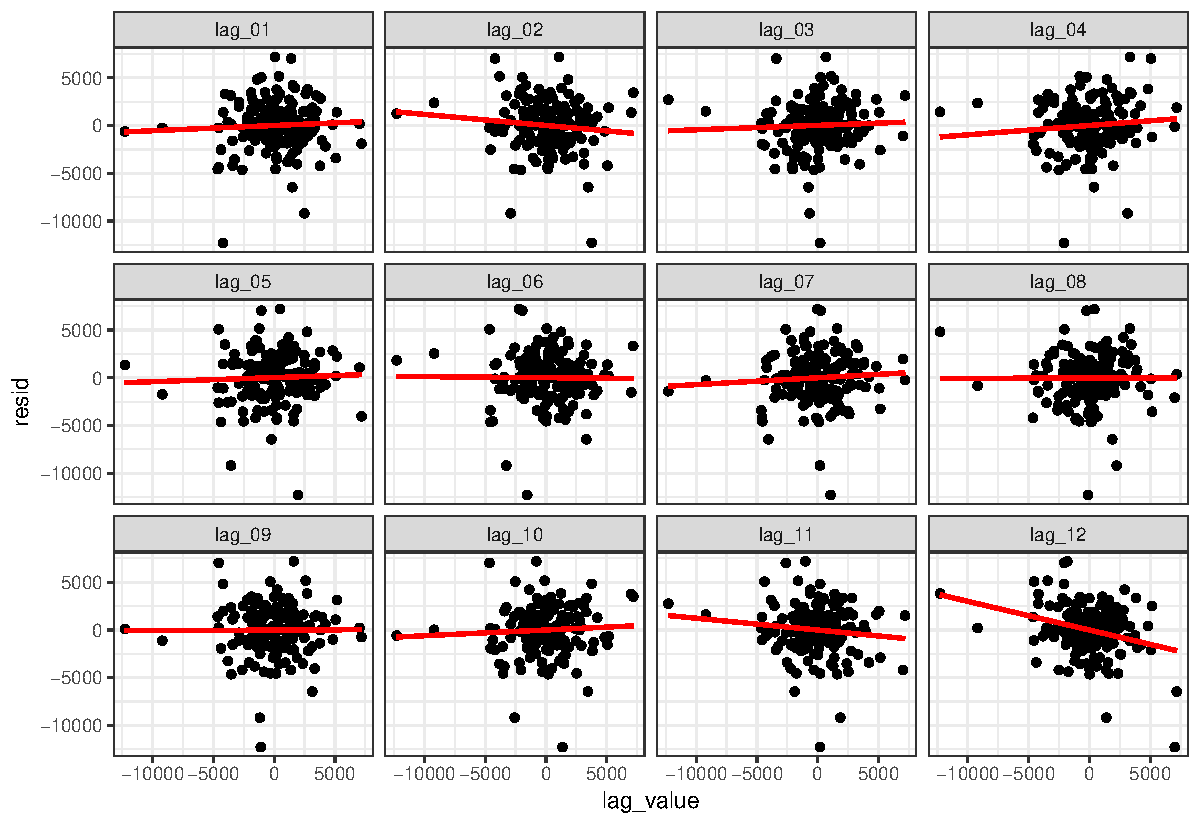
\includegraphics{Lec6_files/figure-beamer/unnamed-chunk-19-1.pdf}

\end{frame}

\begin{frame}[t]{Writing down the model?}

So, is our EDA suggesting that we then fit the following model?

\[ \text{sales}(t) = \beta_0 + \beta_1 \, t + \beta_2 \, t^2 + \beta_3 \, \text{sales}(t-12) + \epsilon_t \]
. . .

the implied model is,

\[ \text{sales}(t) = \beta_0 + \beta_1 \, t + \beta_2 \, t^2 + w_t \]
where

\[ w_t = \delta \, w_{t-12} + \epsilon_t \]

\end{frame}

\end{document}
